\documentclass[11pt]{article}
\usepackage[english]{babel}
\usepackage[utf8x]{inputenc}
\usepackage{amsmath}
\usepackage{graphicx}
\usepackage[colorinlistoftodos]{todonotes}
\usepackage{enumitem}
\usepackage{listings}
\usepackage{filecontents}
\usepackage{verbatim}
\usepackage{eurosym}
\usepackage[export]{adjustbox}
\usepackage{hyperref}

\begin{document}

\begin{titlepage}

\newcommand{\HRule}{\rule{\linewidth}{0.5mm}} % Defines a new command for the horizontal lines, change thickness here

\center % Center everything on the page
 
%----------------------------------------------------------------------------------------
%	HEADING SECTIONS
%----------------------------------------------------------------------------------------

\textsc{\LARGE Concordia University}\\[1.5cm] % Name of your university/college
\textsc{\Large COMP 5531 Files and Databases}\\[0.5cm] % Major heading such as course name
%\textsc{\large Assignment 1}\\[0.5cm] % Minor heading such as course title

%----------------------------------------------------------------------------------------
%	TITLE SECTION
%----------------------------------------------------------------------------------------

\HRule \\[0.4cm]
{ \huge \bfseries Main Project Report \\ Web Career Portal Database}\\[0.4cm] % Title of your document
\HRule \\[1.5cm]
 
%----------------------------------------------------------------------------------------
%	AUTHOR SECTION
%----------------------------------------------------------------------------------------

\begin{minipage}{0.4\textwidth}
\begin{flushleft} \large
\emph{Team ID:} \\ cxc55311 \\
\end{flushleft}
\end{minipage}
~
\begin{minipage}{0.4\textwidth}
\begin{flushright} \large
\emph{Team Members:} \\
Md Tanveer Alamgir \\ ID: 40014877\\
Craig Boucher \\ ID:21295721 \\
Osman Momoh \\ ID: 26220150\\
Fan Zou \\ ID: 40118112\\

\end{flushright}
\end{minipage}\\[2cm]

%\emph{GitHub:} \\ \url{https://github.com/OM234/COMP-5531-Main-Project} \\

% If you don't want a supervisor, uncomment the two lines below and remove the section above
%\Large \emph{Author:}\\
%John \textsc{Smith}\\[3cm] % Your name

%----------------------------------------------------------------------------------------
%	DATE SECTION
%----------------------------------------------------------------------------------------

%{\large \today}\\[2cm] % Date, change the \today to a set date if you want to be precise

%----------------------------------------------------------------------------------------
%	LOGO SECTION
%----------------------------------------------------------------------------------------


\includegraphics[width=50px, keepaspectratio]{Briefcase.png}\\[1cm] % Include a logo
 
%----------------------------------------------------------------------------------------

\vfill % Fill the rest of the page with whitespace

\end{titlepage}

\tableofcontents

\newpage

\section{Introduction}

This project consists of two main components. The design of the database and the website that is used as a tool to implement the database and showcase various features. The database design consisted of creating an entity relation diagram to abstract the database to the core components necessary. This diagram was then used to project the relations that will be required and their associated attributes. From this schema, the functional dependencies were determined and rigorous normalization was performed to ensure the relations were all in at least third normal form. \par
The website, known as the web portal, has a front end to display the user interface and a back-end which connects the functionality between the MySQL database and the front end components. A model-view-controller architecture pattern is used to organize the code in the various files used to build the web portal. \par
The website itself is a career portal interface. There are three types of accounts that have access to the website. Administrators, who have powers to modify other user accounts. Employers, who can post jobs and offer employment. Lastly, job seekers (also known as applicants), can search for job postings and apply to them. There website also handles payment information and payment processing.
\section{Database Design}

The reasonable assumptions made based on the requirements provided in the project description include the following. There will be a table for employers that will contain attributes like the name of the employer, their account category, contact information, username, and password. A table for job seekers (`ordinary' users) to hold data regarding their contact information, account balance, category type, username, and password. A table restricted to administrator accounts will also be necessary. These assumptions were used as a starting point to craft an entity relationship model.

\subsection{Entity-Relation Diagram}

\subsection{E/R Diagram to Relation Conversions}

\subsection{Functional Dependencies}

\subsubsection{Normalization}

\section{Web Portal Functionalities}
Technical languages used: \\
\textit{Programming languages:} JavaScript, PHP, Python \\
\textit{Markup and Stylesheet Languages:} HTML and CSS \\
\textit{Database Management System:} MySQL

\subsection{Software Design \& Architecture}

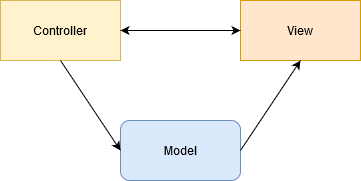
\includegraphics[scale=.7]{MVC.png}

The architectural software design pattern used in the construction of this website is known as Model-View-Controller (MVC). The three interlocking components that perform the core functionality of the website work together to display the interface to the user, gather input from the user, and manage the interaction between the user and the database. The view component displays a graphical interface to the user and receives user input. The controller receives this input and sometimes updates the view directly or manages/manipulates the data requested by the inputs and provides it to the model component. Where the model component, in turn, relays information directly to the view.

\newpage

\subsection{Front-End Development}

Bootstrap, a pivotal framework providing JavaScript and CSS templates was used in the constructions of the front-end. The layout of the website and other visual elements were able to be abstracted away with the Bootstrap framework, making working with the markup and style sheet languages much easier. The functionality for the way users interact with the website was programmed with both JavaScript and PHP.

\subsubsection{Landing Page}

The first page greeting the user is the landing page. Visually, a briefcase image is displayed as a foreground graphic for the website. On landing page a login request is found. A user can proceed to login, create an account, or request a password if they have forgotten their password. \par
When choosing to create a new account the user will be shown a form to enter various information. All of the fields shown are required. Personal data such as name, email,, address, payment information, etc... will be used to create the new account. If a field is left with an invalid input, the user will be notified to correct any missing information. There are slightly different fields depending on which account type (employer, job seeker) the user chooses to create. par
The missing password functionality simply sends a password to the email address that is stored on the account. \par
After entering an appropriate username and password the user will be able to login to the website and progress to the dashboard. The dashboard is different for each type of user: job seeker, employer, and administrator (admin).

\subsubsection{Dashboards}

The two main dashboards used by the most users are the employer and job seeker dashboards. They each provide unique functionalities for the way the user interacts with the website. The third user type, admins, have unique privilege and access to modify the other user accounts directly. An important feature is that if an account is has a negative balance the account becomes deactivated and loses access to most features of the website until they provide a payment to obtain a positive balance. \par
The employer dashboard provides the ability to post jobs, update payment information, hire individuals who applied to job postings, delete/deny the applications of job seekers, upgrade the user category (prime, gold), view status of jobs that have been applied to, view posted jobs, update their contact information, and modify payment features. \par 
The job seeker dashboard provides similar features as the employer dashboard such as updating payment information, personal information, and upgrading or downgrading user categories (basic, prime, gold). There is the ability to search for all of the jobs posted int the database. Once a desired job is found, the job seeker user can apply to the job. All of the jobs that have been applied to will be able to be viewed for status updates and whether to accept or reject (withdraw from) job offers. Lastly, the user may delete their account if desired. \par
The last type of account is the administrator. The admins can activate or deactivate any other user (that is not also an admin).  Every job post is also able to be modified/removed by the admin account.

\subsection{MySQL Database Implementation}

The database management system used is MySQL. A program written in Python was used to generate data to populate the database with. SQL scripts generated by the Python code was then run to create tables and insert the data into the database.

\subsubsection{Generating Data}

A python program was written to generate the data required to fill the database. Everything from phone numbers and email addresses to user names, company names, and credit card numbers were generated using a series of algorithms. Some of the algorithms draw existing data from text files consisting of names, nouns, adjectives, etc... Various forms of primitive data were taken to be used in the algorithms to be combined into data needed to satisfy the attributes belonging to the relations of the database.

\subsubsection{Creating Tables \& Inserting Data}
The files `create\_tables.sql' and `insert\_data.sql' create the database tables and insert the data using SQL queries. The insert data file is generated by the python program. The create table file was written manually based on the database schema provided by the theoretical design work. The primary and foreign keys are clearly implemented in this file.


\subsubsection{SQL Queries}

The file that contains the requested queries is appropriately named `queries.sql'. Some of the queries request merely request the manipulation of one record. Such as deleting a user, inserting a user, obtaining a report of a post posting. All eighteen queries demanded in the main project requirements documented are listed here and labelled with appropriate comments. 


\subsection{Back-End Development}


\subsubsection{Login \& Sign Up}

\subsubsection{Employer Dashboard}

\subsubsection{Job Seeker Dashboard}

\subsubsection{Administrator Dashboard}

\section{CONTRIBUTIONS}

\end{document}